\documentclass[First Project.tex]{subfiles}

\begin{document}
\subsection{ Ιδιοδιάνυσμα μέγιστης ιδιοτιμής ( Μέθοδος των δυνάμεων )}

Σε αυτή την παράγραφο κατασκευάζεται ο πίνακας \textlatin{G} για το υποθετικό μας δίκτυο και υπολογίζεται με την μέθοδο
των δυνάμεων το ιδιοδιάνυσμα που αντιστοιχεί στην μέγιστη ιδιοτιμή του. Ο πίνακα \textlatin{G} είναι ο παρακάτω 

\begin{figure}[h!]
    \centering
    \captionsetup{justification=centering}
    \begin{center}
        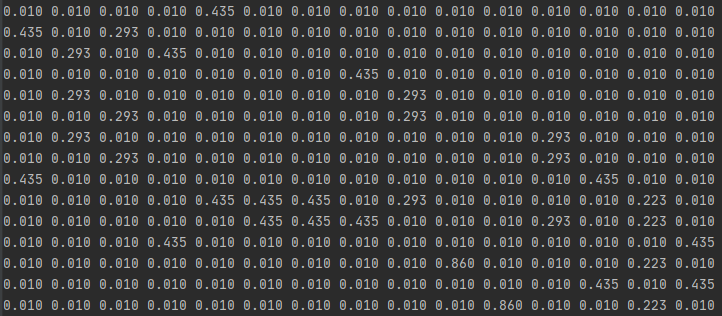
\includegraphics[scale=0.65]{exercise_4_g_matrix.png}    
        \caption{ Ο πίνακας \textlatin{G} για το υποθετικό μας δίκτυο }
    \end{center}
\end{figure} 
\newpage
Αν καλέσουμε την συνάρτηση \textlatin{\textbf{power\_method}} από το αρχείο \textlatin{\textbf{power\_method.py}} όπου
υλοποιείται η μέθοδος των δυνάμεων έχουμε τα παρακάτω αποτελέσματα :
\begin{figure}[h!]
    \centering
    \captionsetup{justification=centering}
    \begin{center}
        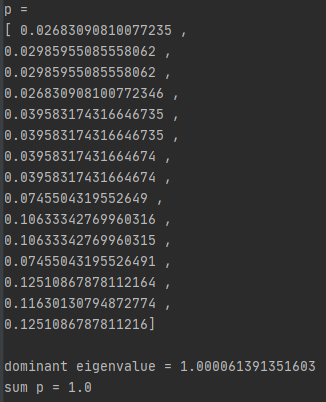
\includegraphics[scale=0.65]{exercise_4_power_method_2.png}    
        \caption{ Αποτελέσματα κλήσης της συνάρτησης \textlatin{power\_method} }
    \end{center}
\end{figure} 

Όπου παρατηρούμε ότι το ιδιοδιάνυσμα που αντιστοιχεί στην μεγαλύτερη ιδιοτιμή, συμφωνεί με αυτό που δίνεται στην εκφώνηση
της άσκησης.
\end{document}